\documentclass[a4paper]{article}
\usepackage[UTF8]{ctex}     %先引入ctex
\usepackage[utf8]{inputenc} %再引入inputenc
\usepackage{graphicx}
% \usepackage{lazylatex}
% \tcbuselibrary{documentation}
\usepackage{amsmath}
\usepackage{amssymb}
\usepackage{bookmark}
\usepackage{enumerate}
\usepackage{geometry}
\usepackage{tikz}
\usepackage{forest}
\usepackage{float}
\usepackage{multirow}
\usepackage{array}
\usepackage{multicol}
\usepackage{listings}
% listings
\definecolor{grey}{rgb}{0.8,0.8,0.8}
\definecolor{darkgreen}{rgb}{0,0.3,0}
\definecolor{darkblue}{rgb}{0,0,0.3}
\lstset{%
    numbers=left, %行号
    numberstyle=\tiny\color{grey},
    showstringspaces=false,
    showspaces=false,%
    tabsize=4,%
    % frame=shadowbox,%
    basicstyle={\ttfamily\scriptsize},%
    keywordstyle=\color{blue!80!black}\bfseries,%
    commentstyle=\color{green!50!blue}\itshape,%
    stringstyle=\color{green!50!black},%
    rulesepcolor=\color{gray!20!white},
    breaklines,
    columns=flexible,
    extendedchars=false,
    %mathescape=true,
    language=c,
}

\graphicspath{{img/}}
% 边距
\geometry{left=2.0cm,right=2.0cm,top=1.0cm,bottom=3.0cm}
% 大题
\newenvironment{problems}{\begin{list}{}{\renewcommand{\makelabel}[1]{\textbf{##1}\hfil}}}{\end{list}}
% 小题
\newenvironment{steps}{\begin{list}{}{\renewcommand{\makelabel}[1]{##1)\hfil}}}{\end{list}}
% 答
\providecommand{\ans}{\textbf{答}:~}
% 解
\providecommand{\sol}{\textbf{解}.~}

\def\slot#1{\framebox(2em,0.75em){#1}}
\def\lab#1{\hbox to 2em{\hfil #1 \hfil}}
\def\heading{\hfill \lab{R1}\lab{R2}\lab{R3}\hspace*{2em}\lab{a}\lab{b}\lab{c}\lab{d}\lab{e}\lab{f}\lab{t}\lab{u}\lab{v}\lab{w}\lab{x}}
\def\headingtwo{\hfill \lab{R1}\lab{R2}\hspace*{2em}\lab{a}\lab{b}\lab{c}\lab{d}\lab{e}\lab{f}\lab{t}\lab{u}\lab{v}\lab{w}\lab{x}}
\begin{document}
\title{\normalsize \underline{编译原理(A)}\\\LARGE第 8 次作业}
\author{Log Creative }
\date{\today}
\maketitle

\begin{problems}
    \item[8.4.1] 简单的矩阵乘法程序。
    \begin{lstlisting}[language=c]
        for (i=0; i<n; i++)
            for (j=0; j<n; j++)
                c[i][j] = 0.0;
        for (i=0; i<n; i++)
            for (j=0; j<n; j++)
                for(k=0; k<n; k++)
                    c[i][j] = c[i][j] + a[i][k]*b[k][j];
    \end{lstlisting}
    \begin{steps}
        \item[1] 假设矩阵的元素是需要 8 个字节的数值,而且矩阵按行存放。把程序翻译为三地址语句。
         
        \sol 
        \begin{multicols}{2}
        \begin{lstlisting}
i = 0
j = 0
t1 = n * i
t2 = t1 + j
t3 = 8 * t2
c[t3] = 0.0
j = j + 1
if j < n goto (3)
i = i + 1
if i < n goto (2)
i = 0
j = 0
t5 = n * i
t6 = t5 + j
t7 = 8 * t6
k = 0
t8 = t5 + k
t9 = 8 * t8
t10 = a[t9]
t11 = n * k
t12 = t11 + j
t13 = 8 * t12
t14 = b[t13]
t15 = t10 * t14
t16 = c[t7]
t16 = t16 + t15
c[t7] = t16
k = k + 1
if k < n goto (17)
j = j + 1
if j < n goto (13)
i = i + 1
if i < n goto (12)
        \end{lstlisting}
        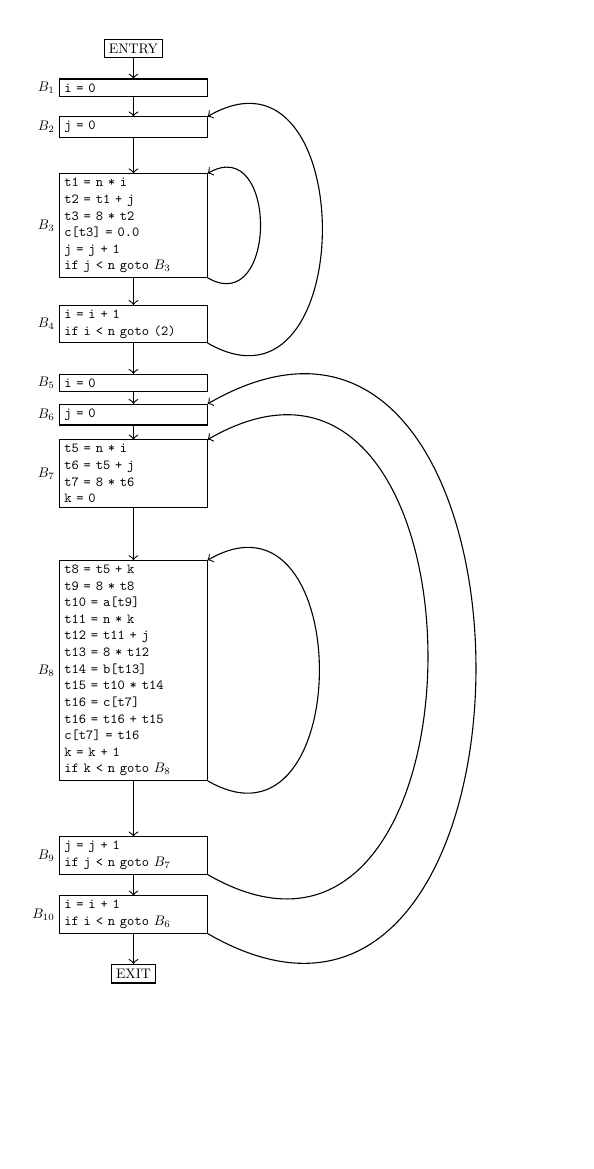
\begin{tikzpicture}[scale=0.5,every node/.style={scale=0.5}]
\tikzstyle{Block}=[draw, text width=10em, font=\ttfamily];
\tikzstyle{seq} = [->];
\tikzstyle{bender} = [bend right, out=-120, in=-60, looseness=2];
\node [Block,label=left:$B_1$] (v1) at (-0.5,2) {i = 0};
\node [Block,label=left:$B_2$] (v2) at (-0.5,1) {j = 0};
\draw [seq] (v1) edge (v2);
\node [Block,label=left:$B_3$] (v3) at (-0.5,-1.5) {\parbox{10em}{
t1 = n * i \\
t2 = t1 + j\\
t3 = 8 * t2\\
c[t3] = 0.0\\
j = j + 1\\
if j < n goto $B_3$}};
\draw [seq] (v2) edge (v3);
\node [Block,label=left:$B_4$] (v4) at (-0.5,-4) {\parbox{10em}{i = i + 1\\
if i < n goto (2)}};
\draw [seq] (v3) edge (v4);
\draw [bender] (v3.south east) edge[->] (v3.north east);
\draw [bender] (v4.south east) edge[->] (v2.north east);
\node [Block,label=left:$B_5$] (v5) at (-0.5,-5.5) {i = 0};
\draw [seq] (v4) edge (v5);
\node [Block,label=left:$B_6$] (v6) at (-0.5,-6.3) {j = 0};
\draw [seq] (v5) edge (v6);
\node [Block,label=left:$B_7$] (v7) at (-0.5,-7.8) {\parbox{10em}{t5 = n * i\\
t6 = t5 + j\\
t7 = 8 * t6\\
k = 0}};
\draw [seq] (v6) edge (v7);
\node [Block,label=left:$B_8$] (v8) at (-0.5,-12.8) {\parbox{10em}{t8 = t5 + k\\
t9 = 8 * t8\\
t10 = a[t9]\\
t11 = n * k\\
t12 = t11 + j\\
t13 = 8 * t12\\
t14 = b[t13]\\
t15 = t10 * t14\\
t16 = c[t7]\\
t16 = t16 + t15\\
c[t7] = t16\\
k = k + 1\\
if k < n goto $B_8$}};
\draw [seq] (v7) edge (v8);
\node [Block,label=left:$B_9$] (v9) at (-0.5,-17.5) {\parbox{10em}{j = j + 1\\
if j < n goto $B_7$}};
\node [Block,label=left:$B_{10}$] (v10) at (-0.5,-19) {\parbox{10em}{i = i + 1\\
if i < n goto $B_6$}};
\draw [seq] (v8) edge (v9);
\draw [seq] (v9) edge (v10);
\draw [bender] (v8.south east) edge[->] (v8.north east);
\draw [bender] (v9.south east) edge[->] (v7.north east);
\draw [bender] (v10.south east) edge[->] (v6.north east);
\node[draw] (v11) at (-0.5,3) {ENTRY};
\node[draw] (v12) at (-0.5,-20.5) {EXIT};
\draw [seq] (v11) edge (v1);
\draw [seq] (v10) edge (v12);
\end{tikzpicture}

        % \begin{figure}
        %     \centering
            
        %     \caption{流图}
        %     \label{fig:fg}
        % \end{figure} 
    \end{multicols}
    \item[2] 为 (1) 中得到的代码构造流图。
    \sol 如上图所示。
     
    \item[3] 找出在 (2) 中得到的流图的循环。 
    \sol \begin{enumerate}
        \item $B_3$ 自身
        \item $\{B_2,B_3,B_4\}$
        \item $B_8$ 自身
        \item $\{B_7,B_8,B_9\}$
        \item $\{B_6,B_7,B_8,B_9,B_{10}\}$
    \end{enumerate}
    
    \end{steps}

    \item[8.6.1] 
    \begin{multicols}{2}
    生成三地址代码
    \begin{verbatim}
        x = a/(b+c) - d*(e+f);
    \end{verbatim} 
    \begin{lstlisting}
t = b + c
u = a / t
v = e + f
w = d * v
x = u - w
    \end{lstlisting}
\end{multicols}
    \item[8.6.3] 把三地址代码转换为本节给出的机器模型的机器代码。假设你有任意多个寄存器可用。
    \begin{lstlisting}
LD R1, b
LD R2, c
ADD R3, b, c
LD R4, a
DIV R5, R4, R3
LD R6, e
LD R7, f
ADD R8, R6, R7
LD R9, d
MUL R10, R9, R8
SUB R11, R5, R10
ST x, R11
    \end{lstlisting} 
    \item[8.6.4] 假设有三个可用的寄存器,使用本节中的简单代码生成算法,转换为机器代码。请给出每一个步骤之后的寄存器和地址描述符。
    \sol

{\ttfamily
        \heading

        \hfill \slot{}\slot{}\slot{}\hspace*{2em}\slot{a}\slot{b}\slot{c}\slot{d}\slot{e}\slot{f}\slot{}\slot{}\slot{}\slot{}\slot{}
        
        \begin{verbatim}
t = b + c
    LD R1, b
    LD R2, c
    ADD R1, R1, R2
        \end{verbatim}

        \heading

        \hfill \slot{t}\slot{c}\slot{}\hspace*{2em}\slot{a}\slot{b}\slot{c,R2}\slot{d}\slot{e}\slot{f}\slot{R1}\slot{}\slot{}\slot{}\slot{}

        \begin{verbatim}
u = a / t
    LD R2, a
    DIV R1, R2, R1
        \end{verbatim}

        \heading

        \hfill \slot{u}\slot{a}\slot{}\hspace*{2em}\slot{a,R2}\slot{b}\slot{c}\slot{d}\slot{e}\slot{f}\slot{}\slot{R1}\slot{}\slot{}\slot{}

        \begin{verbatim}
v = e + f
    LD R2, e
    LD R3, f
    ADD R2, R2, R3
        \end{verbatim}

        \heading

        \hfill \slot{u}\slot{v}\slot{f}\hspace*{2em}\slot{a}\slot{b}\slot{c}\slot{d}\slot{e}\slot{f,R3}\slot{}\slot{R1}\slot{R2}\slot{}\slot{}

        \begin{verbatim}
w = d * v
    LD R3, d
    MUL R2, R2, R3
        \end{verbatim}

        \heading

        \hfill \slot{u}\slot{w}\slot{d}\hspace*{2em}\slot{a}\slot{b}\slot{c}\slot{d,R3}\slot{e}\slot{f}\slot{}\slot{R1}\slot{}\slot{R2}\slot{}

 \begin{verbatim}
x = u - w
    SUB R1, R1, R2
\end{verbatim}
    
        \heading

        \hfill \slot{x}\slot{w}\slot{d}\hspace*{2em}\slot{a}\slot{b}\slot{c}\slot{d,R3}\slot{e}\slot{f}\slot{}\slot{}\slot{}\slot{R2}\slot{R1}

\begin{verbatim}
    ST x, R1
\end{verbatim}

        \heading

        \hfill \slot{x}\slot{w}\slot{d}\hspace*{2em}\slot{a}\slot{b}\slot{c}\slot{d,R3}\slot{e}\slot{f}\slot{}\slot{}\slot{}\slot{R2}\slot{x,R1}
}
    \item[8.6.5] 重复练习 8.6.4,但是假设只有两个可用的寄存器。
    \sol

{\ttfamily

\headingtwo

\hfill \slot{}\slot{}\hspace*{2em}\slot{a}\slot{b}\slot{c}\slot{d}\slot{e}\slot{f}\slot{}\slot{}\slot{}\slot{}\slot{}

\begin{verbatim}
t = b + c
    LD R1, b
    LD R2, c
    ADD R1, R1, R2
\end{verbatim}

\headingtwo

\hfill \slot{t}\slot{c}\hspace*{2em}\slot{a}\slot{b}\slot{c,R2}\slot{d}\slot{e}\slot{f}\slot{R1}\slot{}\slot{}\slot{}\slot{}

\begin{verbatim}
u = a / t
    LD R2, a
    DIV R1, R2, R1
\end{verbatim}

\headingtwo

\hfill \slot{u}\slot{a}\hspace*{2em}\slot{a,R2}\slot{b}\slot{c}\slot{d}\slot{e}\slot{f}\slot{}\slot{R1}\slot{}\slot{}\slot{}

\begin{verbatim}
    ST u, R1
\end{verbatim}

\headingtwo

\hfill \slot{u}\slot{a}\hspace*{2em}\slot{a,R2}\slot{b}\slot{c}\slot{d}\slot{e}\slot{f}\slot{}\slot{u}\slot{}\slot{}\slot{}

\begin{verbatim}
v = e + f
    LD R1, e
    LD R2, f
    ADD R1, R1, R2
\end{verbatim}

\headingtwo

\hfill \slot{v}\slot{f}\hspace*{2em}\slot{a}\slot{b}\slot{c}\slot{d}\slot{e}\slot{f,R2}\slot{}\slot{u}\slot{R1}\slot{}\slot{}

\begin{verbatim}
w = d * v
    LD R2, d
    MUL R1, R1, R2
\end{verbatim}

\headingtwo

\hfill \slot{w}\slot{d}\hspace*{2em}\slot{a}\slot{b}\slot{c}\slot{d,R2}\slot{e}\slot{f}\slot{}\slot{u}\slot{}\slot{R1}\slot{}

\begin{verbatim}
x = u - w
    LD R2, u
    SUB R1, R2, R1
\end{verbatim}

\headingtwo

\hfill \slot{x}\slot{u}\hspace*{2em}\slot{a}\slot{b}\slot{c}\slot{d}\slot{e}\slot{f}\slot{}\slot{u,R2}\slot{}\slot{}\slot{R1}

\begin{verbatim}
    ST x, R1
\end{verbatim}

\headingtwo

\hfill \slot{x}\slot{u}\hspace*{2em}\slot{a}\slot{b}\slot{c}\slot{d,R3}\slot{e}\slot{f}\slot{}\slot{u,R2}\slot{}\slot{}\slot{x,R1}
}
\end{problems}

\end{document}
